\documentclass{article}

% Language setting
% Replace `english' with e.g. `spanish' to change the document language
\usepackage[english]{babel}

% Set page size and margins
% Replace `letterpaper' with`a4paper' for UK/EU standard size
\usepackage[letterpaper,top=2cm,bottom=2cm,left=3cm,right=3cm,marginparwidth=1.75cm]{geometry}

% Useful packages
\usepackage{amsmath}
\usepackage{graphicx}
\usepackage{tcolorbox}
\usepackage{float}

\usepackage[colorlinks=true, allcolors=blue]{hyperref}

\title{Exerices interactifs}
\author{Les bgs de la physique}

\begin{comment}
Question: [...]
\begin{enumerate}
    \item ...
    \item ...
    
\end{enumerate}
\end{comment}

\begin{document}
\maketitle

\section{Maths I}
\begin{enumerate}
    \item Lors de la Welcome Party, vous participez à une course relais avec votre groupe de coaching. Votre camarade a pris du retard que vous devez rattraper. Vous savez que la vitesse nécessaire en fonction du temps s’écrit ainsi : \[v(t) = a e^{-t/b}-bc \]
où $t$ le temps et $a,b$ et $c$ des constantes. Trouver $\Dot{v}$ (la dérivée de la vitesse par rapport au temps).

    \begin{itemize}
        \item $\Dot{v} = -ab e^{-\frac{t}{b}}-bct +d$
        \item $\Dot{v} =- (\frac{a}{b})e^{-\frac{t}{b}}$ %bonne reponse
        \item $\Dot{v} =- (\frac{a}{b})e^{-\frac{t}{b}}-bc$
        \item $\Dot{v} = (\frac{a}{b})e^{-\frac{t}{b}}$ 
    \end{itemize}
    
    \item Maintenant que vous avez trouvé l'accélération, trouver l'équation horaire (la formule de la position) associé à cette vitesse
    
    \begin{itemize}
        \item  $x(t) = -abe^{-\frac{t}{b}}-bct +d$
        \item $x(t) = -abe^{-\frac{t}{b}}-bct $
        \item $x(t) = abe^{-\frac{t}{b}}-bct +d$
        \item $x(t) = -abe^{-\frac{t}{b}}-bc +d$

    \end{itemize}

    \item Soit $\phi(t)$ une fonction qui représente l'angle $\phi$ d'une point par rapport au temps. Que vaut l'expression suivante:
    \[ \frac{d}{dt}(sin^2(\Dot{\phi}))\] %forme (f(g(h(t)))
    \begin{itemize}
        \item $\Ddot{\phi} \; \sin{2 \Dot{\phi}}$ %réponse correcte (je crois lel)
        \item $\sin{(2 \Dot{\phi})}$ %oubli de la seconde dérivée interne
        \item $ 2\Ddot{\phi} \; \cos{\Dot{\phi}} $ %oublie de la première derivee interne
        \item $2 \Ddot{\phi} \; \sin{\Dot{\phi}}$
    \end{itemize}
    
    
    \item  Soient 2 vecteurs u et v dans un  repère cartésien direct (O,x,y,z) : $\Vec{u} = (b,0,a)$ et $\Vec{v} = (bsin(c),-bcosc,a)$ (avec a,b et c des constantes). Que doivent valoir a,b,c pour que $\Vec{u} \cdot \Vec{v} =0 $ ? 
    \begin{itemize}
        \item a=0, b=1, c=$\pi$  %bonne
        \item peu importe les valeurs de a,b,c
        \item a=0, b=5, c=$\dfrac{\pi}{2}$
        \item a=0, b=1, c=\dfrac{\pi}{2}
        
    \end{itemize}
    % et si tu mettais un truc du style : Que faut-il faire pour que ces vecteurs soient perpendiculaires : -a=1, b=2, c=pi
    %peu improte a,b,c etc, comme ça ils réfléchissent à tout ça plutot que faire un bête calcul. 
    \item Que vaut $\Vec{a} \times \Vec{a}$ ?
    \begin{itemize}
        \item $ \lVert \Vec{a} \rVert ^2$
        \item Cette opération n'est pas définie
        \item Cela dépend de la norme de $\Vec{a}$
        \item $\Vec{0}$
    \end{itemize}
    
    \item Que vaut $\Vec{b} \times \Vec{a}$
    \begin{itemize}
        \item $\Vec{0}$
        \item $- \Vec{a} \times \Vec{b}$
        \item $\Vec{a} \times \Vec{b}$
        \item Cela dépend
    \end{itemize}
    
    \item Dans cette situation, projetez le vecteur poids $\Vec{P}$ sur les axes $x$ et $y$:
    \begin{figure}[H]
        \centering
        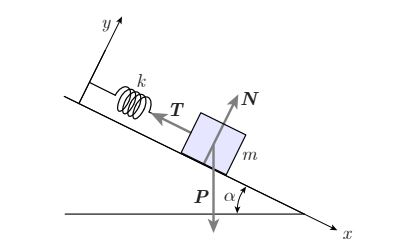
\includegraphics[]{Images/projections_kahoot.JPG}
        %\caption{Caption}
        \label{fig:proj_k}
    \end{figure}
    \begin{itemize}
        \item $\textbf{P} = P\;(\sin{\alpha} \; \hat{\textbf{x}} - \cos{\alpha} \; \hat{\textbf{y}})$ %réponse correcte
        \item $\textbf{P} = P\;(\cos{\alpha} \; \hat{\textbf{x}} + \sin{\alpha} \; \hat{\textbf{y}})$
        \item $\textbf{P} = P\;(\cos{\alpha} \; \hat{\textbf{x}} - \sin{\alpha} \; \hat{\textbf{y}})$
        \item $\textbf{P} = P\;(\sin{\alpha} \; \hat{\textbf{x}} + \cos{\alpha} \; \hat{\textbf{y}})$
    \end{itemize}
    
    


\end{enumerate}
\section{Maths II}

\begin{enumerate}

    \item Trouver une approximation linéaire de tan(x) autour de x = 0:
    \begin{itemize}
        \item $f(x) = \frac{1}{x}$
        \item $f(x) = 1 + x$
        \item $f(x) = x$ %bonne réponse
        \item $f(x) = x + \frac{x^3}{3}$
    \end{itemize}
    
    \item Pour trouver les constantes d'intégrations d'une équation différentielle, on utilise:
    \begin{itemize}
        \item Cela va dépendre du type d'équations différentielles
        \item Les conditions initiales
        \item Cela importe peu, on peut leur donner une valeur arbitraire (souvent 0)
        \item Les valeurs de $f'(0)$ et $f''(0)$
    \end{itemize}
    
\end{enumerate}

%v/f est ce une equa diff

%donner approx lin d'une fonction en un point


\section{Méca I}

\begin{enumerate}

    \item Un bloc glisse à vitesse constante sur un plan horizontal. Quelles sont les forces s'exerçant sur le bloc ? On néglige les forces de frottement
    \begin{itemize}
        \item Aucunes
        \item Une force horizontale \textbf{F} qui le fait avancer
        \item Son poids \textbf{P} et la force de réaction normale du plan \textbf{N} %Réponse correcte
        \item Son poids \textbf{P}, la force de réaction normale du plan \textbf{N} et une force horizontale \textbf{F} qui le fait avancer
    \end{itemize}
    
    \item Dans le référentiel du sol terrestre, laquelle des propositions suivantes est fausse:
    \begin{itemize}
        \item $\frac{d\Vec{p}}{dt} = \sum \Vec{F}^{ext}$
        \item Si un objet est en MRU, alors $\sum \Vec{F}^{ext} = \Vec{0}$
        \item $m \Vec{a}= \sum \Vec{F}^{ext}$ %Faux, il n'est pas précisé que m est constant
        \item $\Vec{F}^{a \rightarrow b} = -\Vec{F}^{b \rightarrow a}$ % 3eme loi
    \end{itemize}
    
    \item Une balle est lancée verticalement vers le haut. Qualifiez sa vitesse et son accélération au point le plus haut de sa trajectoire (on néglige les frottements):
    \begin{itemize}
        \item La vitesse est maximal et l'accélération est nulle
        \item La vitesse est nulle et l'accélération est nulle
        \item La vitesse est nulle et l'accélération est croissante
        \item La vitesse est nulle et l'accélération est une constante %bonne reponse
    \end{itemize}

    \item (V/F) L'équation horaire d'une bille qui chute avec une vitesse initiale $v_0$ et une position initiale $x_0$ (on ne considère pas les frottements) est de la forme $x(t) = \frac{1}{2}gt^2+v_0t+x_0$
    %Faux, signe moins manquant
\end{enumerate}

    
\section{Méca II}

\begin{enumerate}


    \item (voir image) On considère un pendule incliné d'un point matériel de masse $m$ est contraint de se déplacer sur un cercle de rayon $R$ contenu sur un plan incliné d'un angle $\alpha$ par rapport au plan horizontal. Quels types de coordonnées privilégieriez vous ?
    \begin{figure}[H]
        \centering
        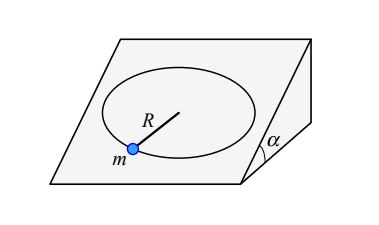
\includegraphics[]{Images/penduleincline.JPG}
        %\caption{Caption}
        \label{fig:penduleincl}
    \end{figure}
    \begin{itemize}
        \item Les coordonnées cartésiennes
        \item Les coordonnées cylindriques %réponse correct
        \item Les coordonnées sphériques
        \item Aucun des coordonnées vues en cours conviennent ici
    \end{itemize}
    
    \item Dans un repère cylindrique, le vecteur position du point $M$ est donné par:
    \begin{itemize}
        \item $\Vec{OM} = r \Vec{e}_r$
        \item $\Vec{OM} = \theta \Vec{e}_{\theta} + z \Vec{e}_z$
        \item $\Vec{OM} = r \Vec{e}_r + z \Vec{e}_z$ %bonne réponse
        \item $\Vec{OM} = r \Vec{e}_r + \theta \Vec{e}_{\theta} + z \Vec{e}_z$
        
    \end{itemize}
    
    
    \begin{comment}
    
    Une voiture de course roule à une vitesse horizontale de norme $v$ constante sur un circuit circulaire de rayon $R$. La piste est inclinée d’un angle $\alpha$ par rapport à l'horizontale (pour que la voiture soit penchée vers l’intérieur du virage).

    \begin{figure}[]
        \centering
        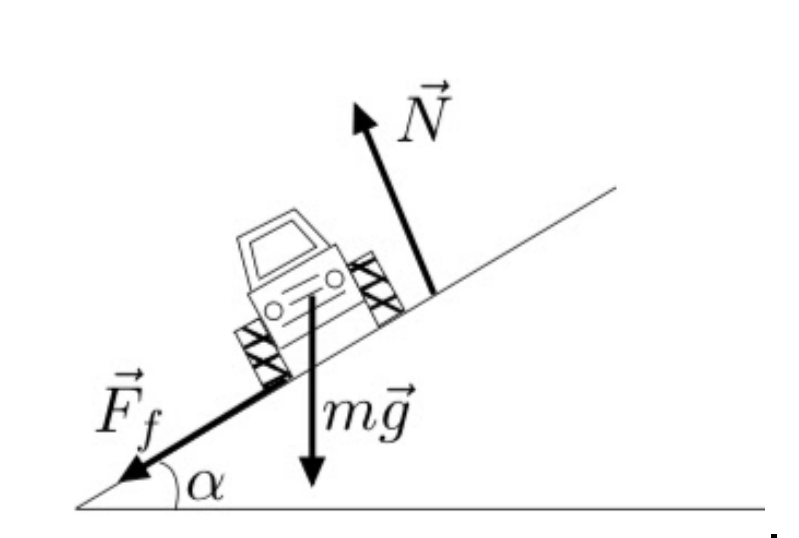
\includegraphics[H]{Images/voiture.png}
        %\caption{Caption}
        \label{fig:my_voiture}
    \end{figure}
    
    \end{comment}
    
    \item Considérons un oscillateur harmonique ayant pour solution \[x(t) = A \cos{(\omega t + \phi)} \]
    Lequel des suivants est correct ? 
    \begin{itemize}
        \item A correspond à l'amplitude, $\omega$ la pulsation et $\phi$ le déphasage %réponse correcte
        \item A correspond à l'amplitude, $\omega$ le déphasage  et $\phi$ la pulsation
        \item A correspond au déphasage, $\omega$ la pulsation et $\phi$ l'amplitude
        \item A correspond au déphasage, $\omega$ l'amplitude et $\phi$ la pulsation
    \end{itemize}
    
    \item (V/F) L'équation différentielle $m \Ddot{x} = kx$ est une équation différentielle représentant un oscillateur harmonique ($m > 0$ et $k > 0$) .
    %Faux il manque le signe moins
\end{enumerate}

\end{document}